%
% Main thesis LaTeX file. We use the REPORT style format
% instead of article for most technical papers
%
%
\documentclass[12pt,fleqn]{article}

%%%%%%%%%%%%%%%%%%%%%%%%%%%%%%%%%%%%%%%%%%%%%%%%%%%%%%%%%%%%%%%%%%%%
%
% list the set of packages we use for various aspects of 
% the thesis format
%
\usepackage{layout}
\usepackage[utf8]{inputenc}
\usepackage{setspace}

\usepackage{subfigure}
\usepackage{epsfig}
\usepackage{float}
\usepackage{floatflt}
\usepackage{listings}
\usepackage{palatino}
\usepackage{verbatim}
\usepackage{footnpag}
\usepackage{caption}
\usepackage[mathcal, mathbf]{euler}
\usepackage{amsmath}
\usepackage{amstext}
\usepackage{color}
\usepackage{xcolor}
\usepackage{graphicx}


%%%%%%%%%%%%%%%%%%%%%%%%%%%%%%%%%%%%%%%%%%%%%%%%%%%%%%%%%%%%%%%%%%%%
%
% include two local LaTeX source files that establish the
% thesis layout and the set of additional commands we find
% useful for creating the text.
%
\input{layout}
\input{newcommands}
\input{outline_support}


\newcommand{\Organization}{School of Computer Engineering}

\title{CE2004: Circuits \& Signal Analysis Part 1}

\author{
  Lu Shengliang \\
  SLU001\\
  \Organization{} \\
  \vspace*{-10mm} \\
  Nanyang Technological University \\
  \vspace*{-10mm} \\
  SLU001@e.ntu.edu.sg
}

%
% This begins the actual lab report
%
\renewcommand{\OutlineLevel}{2}

\begin{document}

\maketitle

\begin{abstract}
\ls{1}
\emph{lab 1}: verify the circuit analysis techniques – Ohm Law, KCL, KVL experimentally. \emph{lab 2}: verify the circuit analysis techniques - Superposition and Thévenin’s Theorems, experimentally.
\ls{1.2}
\end{abstract}

\ls{1.2}

\section{lab 1}
\subsection{Introduction}
%=====================================================================
KVL states that the sum of the voltages in a closed loop in a circuit is zero when voltage polarities are properly taken into consideration. \\
KCL states that the sum of the currents entering a point in a circuit at any instant equals the sum of the currents leaving that point. \\
The measurement method is shown in Figure 1.\\
\begin{figure}[H]
\centering
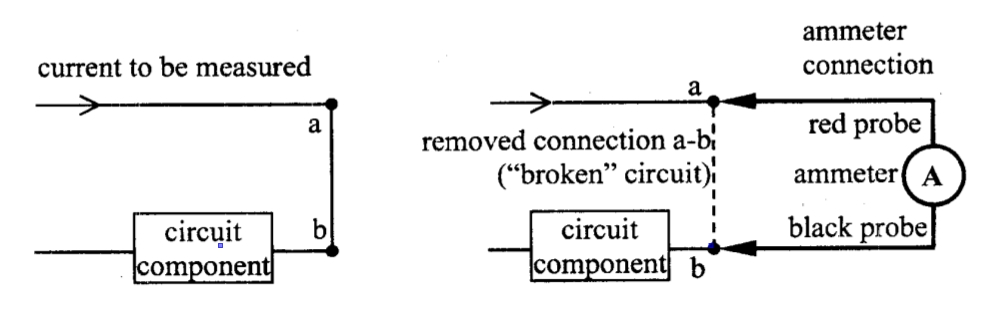
\includegraphics[width=\textwidth]{1.jpg}
\caption{Voltage and Current measurement}
\end{figure}
%=====================================================================
\subsection{Experiments and Results}
\begin{figure}[H]
\centering
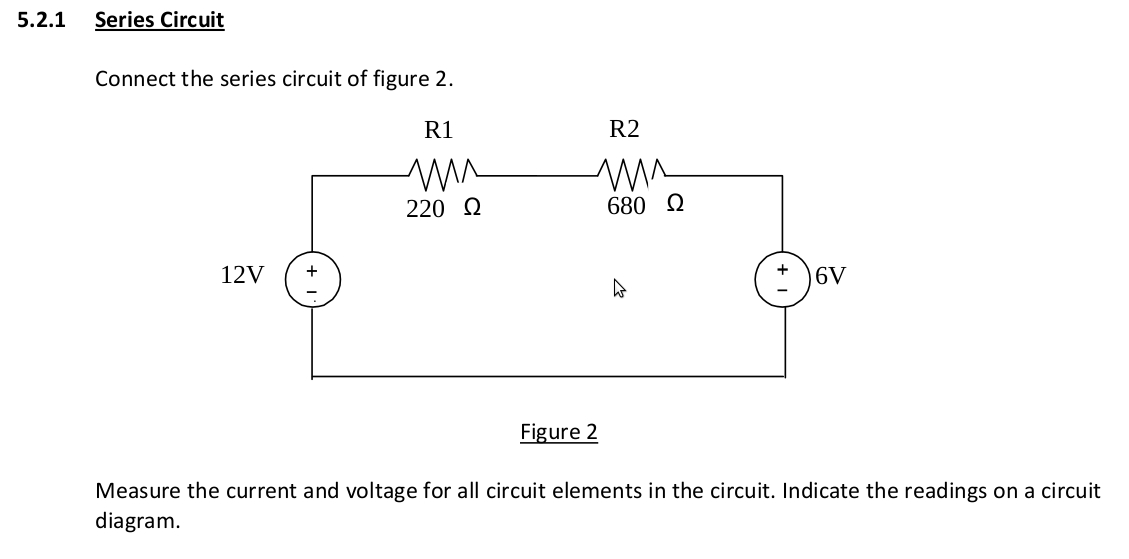
\includegraphics[width=\textwidth]{2.jpg}
\caption{lab1-5.2.1}
\end{figure}
\begin{table}[H]
  \centering
  \begin{tabular}{| c | c | c | l |}
    \hline
    \textbf{Circuit Elements} & \textbf{Current} & \textbf{Voltage} & \textbf{Power} \\ \hline
    12V Voltage Source & 6.579mA & -11.936V & 78.290mW \\
    \hline
    6V Voltage Source & 6.583mA & 6.117V & 40.156mW \\
    \hline
    R1 & 6.574mA & 1.446V & 9.506mW \\
    \hline
    R2 & 6.615mA & 4.519V & 29.893mW \\
    \hline
  \end{tabular}
  \caption{lab1-5.2.1}
\end{table}
Since 12V voltage source is greater than 6V voltage source, with opposite voltage polarities. The real voltage polarity in the circuit should be the same as the 12V one. It results that the current direction is clockwise.
\textbf{Lab 1 Question 1:}
\\The resistors used in the lab are typically rated at 0.25 W. What is the maximum current that can be allowed in (a) R1, (b) R2 and (c) the given circuit?\\
\textbf{Lab 1 Answer 1:}
\begin{gather}
P = \frac{I^2}{R}\\
P \leq 0.25W\\
I \leq \sqrt{P*R}\\
R1(a) : I \leq {0.25W * 220\Omega} = 33.710mA\\
R2(b) : I \leq {0.25W * 680\Omega} = 19.174mA\\
Circuit(c) : \emph{Min}\{R1(a), R2(b)\} = 19.174mA
\end{gather}
\begin{figure}[H]
\centering
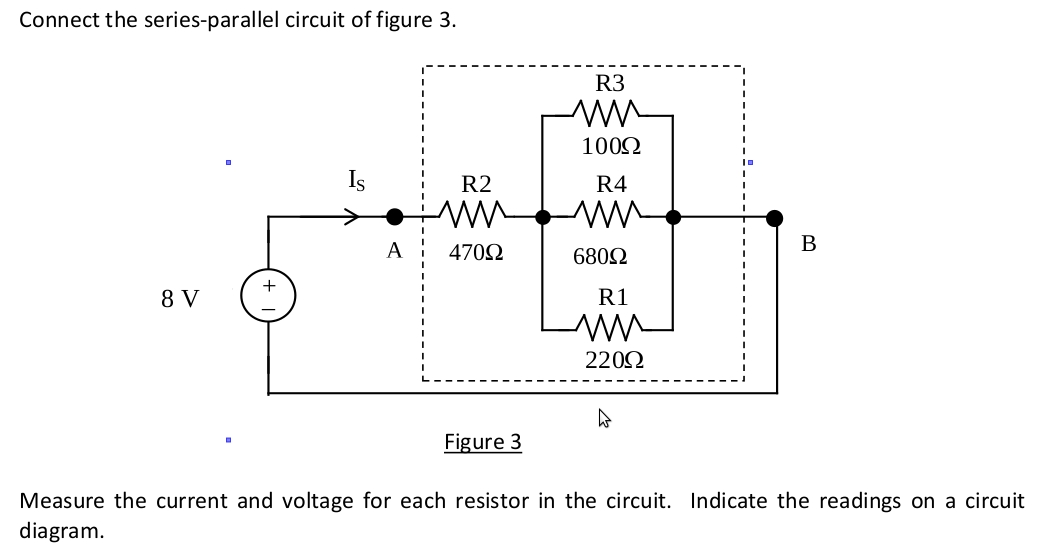
\includegraphics[width=\textwidth]{3.jpg}
\caption{lab1-5.2.2}
\end{figure}
\begin{table}[H]
  \centering
  \begin{tabular}{| c | c | c |}
    \hline
    \textbf{Resistor} & \textbf{Current} & \textbf{Voltage}\\
    \hline
    R1 220\ensuremath{\Omega} & 4.583mA & 1.051V \\
    \hline
    R2 470\ensuremath{\Omega} & 14.745mA & 7.049V \\ 
    \hline
    R3 100\ensuremath{\Omega} & 9.970mA & 1.051V \\
    \hline
    R4 680\ensuremath{\Omega} & 1.513mA & 1.050V \\
    \hline
  \end{tabular}
  \caption{lab1-5.2.2}
\end{table}
\textbf{Lab 1 Question 2:}
\\1) From the measurements made, determine the resistance between terminals A-B of the given circuit. Verify your answer through calculation using the known circuit configuration and resistor values.\\
2) If all resistors between terminals A-B are allowed to be connected in any configuration except for four resistors in parallel, re-arrange the resistors so that the current $I_S$ is maximum. What is this maximum value of $I_S$?\\
\textbf{lab 1 Answer 2:}
\begin{gather}
1)  R_{AB} = 540.781\Omega \\
2)  \frac{1}{\frac{1}{100\Omega} + \frac{1}{470\Omega + 680\Omega} + \frac{1}{220\Omega}} = 64.872\Omega \\
3)  I_S = \frac{8V}{64.872\Omega} = 0.123A
\end{gather}
The method is arranging 470\ensuremath{\Omega}, 680\ensuremath{\Omega} in series, and then connect it with 220\ensuremath{\Omega} and 100\ensuremath{\Omega} in parallel. The maximum value of $I_S$ is 0.123A.
\subsection{Conclusion}
\textbf{Part 1}: a series circuit is under measurement, in order to observe KVL.
\textbf{Part 2}: a series-parallel circuit is seted up and under Measurement, in order to observe KCL and Ohm's law.
%=====================================================================
\section{lab 2}
\subsection{Introduction}

The Superposition Theorem states that the current or voltage associated with a branch in a linear network equals to the sum of the current or voltage components set up in that branch due to each of the independent sources acting one at a time on the circuit.\\
Thevenin's theorem enables us to replace the fixed portion of the circuit by a greatly simplified equivalent circuit. This reduces the complexity of computations required to determine the response in the load circuit when the load changes. The Thevenin’s equivalent circuit consists of a voltage source $V_{TH}$ in series with a resistor $R_{TH}$ as shown:
\begin{figure}[H]
\centering
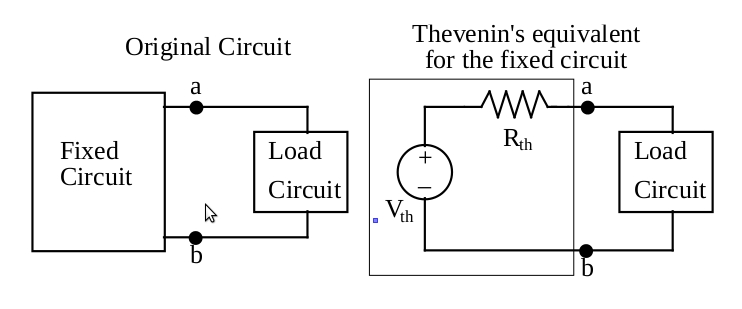
\includegraphics[width=\textwidth]{4.jpg}
\caption{lab2-4.2}
\end{figure}

\subsection{Experiments and Results}

\begin{figure}[H]
\centering
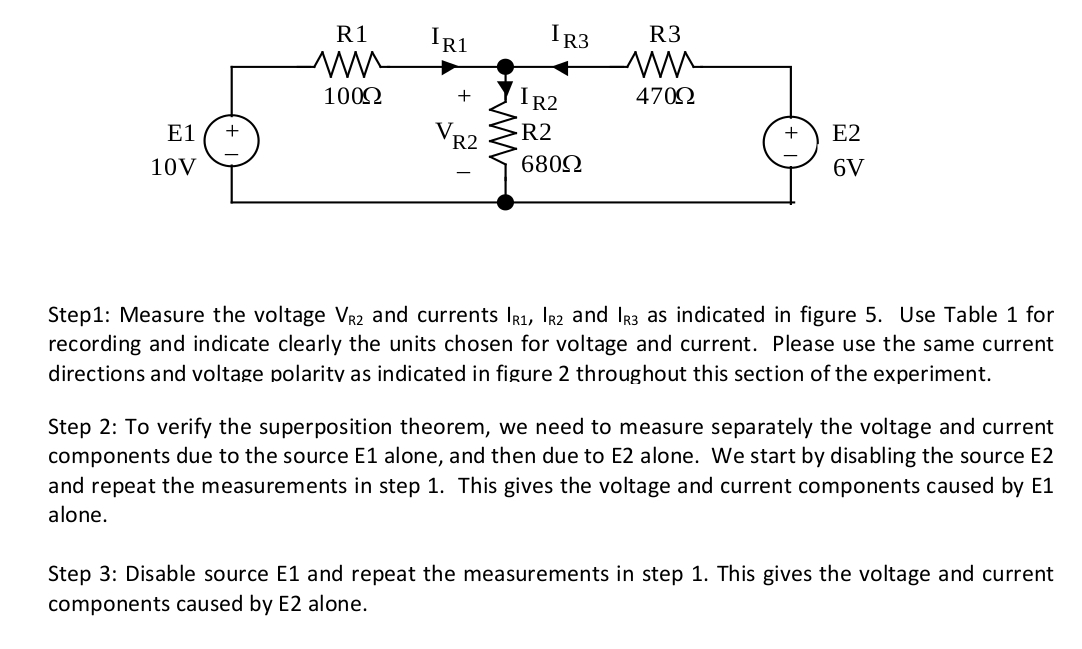
\includegraphics[width=\textwidth]{5.jpg}
\caption{lab2-5.1}
\end{figure}


\begin{table}[H]
  \centering
  \begin{tabular}{| c | c | c | c | c |}
    \hline
    \textbf{Source} & \textbf{$V_{R2}$} & \textbf{$I_{R1}$} & \textbf{$I_{R2}$} & \textbf{$I_{R3}$} \\
    \hline
    E1 \& E2 & 8.36V & 17.03mA & 12.14mA & -5.01mA \\
    \hline
    E1 & 7.31V & 25.74mA & 10.74mA & -15.58mA \\ 
    \hline
    E2 & 0.92V & -9.05mA & 1.33mA & 10.49mA \\
    \hline
  \end{tabular}
  \caption{lab2-5.1}
\end{table}
\textbf{Lab 2 Question 1:}
\\Did you encounter any negative current or voltage in your measurement? If yes, what do these results mean?\\
\textbf{Lab 2 Answer 1:}
\\Yes.\\
The negative sign means the direction of a certain current is opposite from the current meter measurement. 

\begin{figure}[H]
\centering
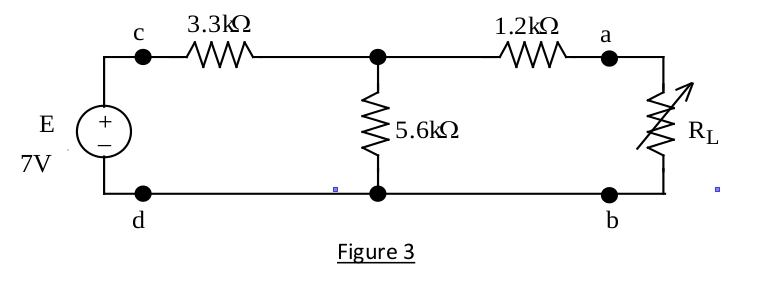
\includegraphics[width=\textwidth]{6.jpg}
\caption{lab2-5.2.1}
\end{figure}
i) Connect the circuit without the load resistor $R_L$(o/s \textbf{a-b}). Measure the input Voltage, E, at the terminals \textbf{c-d}. Make sure the voltage is \emph{7.00V}.\\
ii) Measure the voltage at the terminals \textbf{a-b}, which is $V_{TH}$ = \emph{4.42V}.\\
iii) Short circuit the terminals \textbf{a-b} and measure the current flowing from terminal \textbf{a} to terminal \textbf{b}, which is $I_{TH}$ = \emph{1.34mA}.\\
iv)
\begin{equation}\\R_{TH} = \frac{V_{TH}}{I_{TH}} = \frac{4.42V}{1.34mA} = 3.30K\ensuremath{\Omega}\end{equation}
v) Remove short circuit across \textbf{a-b} and voltage source, and then short circuit \textbf{c-d}. Measure the resistance at the terminals \textbf{a-b}.
\begin{equation}
\\R^\prime_{TH} = 3.28K\Omega \approx R_{TH}
\end{equation}
vi) Connect different load resistors $R_L$ at the terminals \textbf{a-b}. Measure the voltage across $R_L$ and calculate the current through it.

\begin{table}[H]
  \centering
  \begin{tabular}{| c | c | c |}
    \hline
    \textbf{Resistor} & \textbf{Voltage} & \textbf{Current} \\
    \hline
    1 k\ensuremath{\Omega} & 1.04V & 1.04mA \\
    \hline
    4.7 K\ensuremath{\Omega} & 2.60V & 0.55mA \\
    \hline
    10 K\ensuremath{\Omega} & 3.35V & 0.34mA \\
     \hline
  \end{tabular}
  \caption{lab2-5.2.1}
\end{table}

vii) Using the circuit below and repeat the measurements.\\
\begin{figure}[H]
\centering
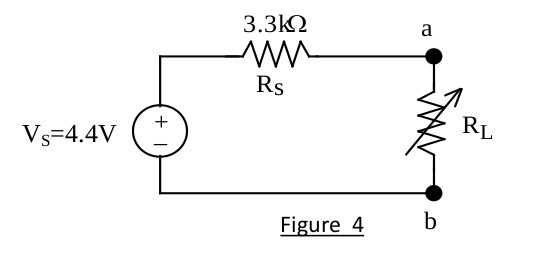
\includegraphics[width=0.8\textwidth]{7.jpg}
\caption{lab2-5.2}
\end{figure}


\begin{table}[H]
  \centering
  \begin{tabular}{| c | c | c |}
    \hline
    \textbf{Resistor} & \textbf{Voltage} & \textbf{Current} \\
    \hline
    1 k\ensuremath{\Omega} & 1.02V & 1.03mA \\
    \hline
    4.7 K\ensuremath{\Omega} & 2.58V & 0.54mA \\
    \hline
    10 K\ensuremath{\Omega} & 3.30V & 0.33mA \\
    \hline
  \end{tabular}
  \caption{lab2-5.2.2}
\end{table}
Table 4 and Table 5 shows that the second circuit is the expected circuit for the original circuit. To find the Thevenin’s equivalent circuit, first disconnect the load circuit from the terminals \textbf{a-b} and then follow by measuring the voltage in the fixed circuit at the terminals \textbf{a-b}. This gives the Thevenin’s equivalent voltage $V_{TH}$. The next step is to disable all the independent sources in the fixed circuit and measure the resistance at the terminals \textbf{a-b}. This gives the Thevenin’s equivalent resistance $R_{TH}$. Then if a $V_{TH}$ voltage source and a $R_{TH}$ resistor is connected with $R_L$. It will behave then same as the original circuit.
\subsection{Discussions}
\textbf{Part 1}: Open circuit two voltage sources one by one, and then compare the data with originally measured data.
\textbf{Part 2}: Thevenin's theorem is enables us to replace the fixed portion of the circuit by a greatly simplified equivalent circuit, which is obsered buy using $R_{TH}$ and $V_{TH}$ to reset up Thevenin's equivalent circuit.


\section{Discussions}
One common mistake is using wrong resistors during circuit set-up section. Choosing correct resistors is required for a correct result. A simple and clear circuit is helpful for mistake detection.

%\section{lab 3}
%\subsection{Introduction}
%In this experiment, an alternating current(AC)--square wave--voltage supply to charge the capacitor through the resistor many times per second, first in a positive direction and then in a negative direction. The charging process also exhibits the same exponential behaviour as the discharge. However during charging progress, the the exponential curve approaches a constant asymptotic value rather than a zero value.
%\begin{figure}[H]
%\centering
%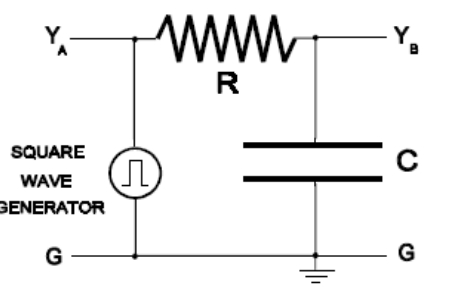
\includegraphics[width=0.6\textwidth]{8.jpg}
%\caption{lab3-5.1}
%\end{figure}

%Connecting the $Y_A$ and $Y_B$ channels of the Oscilloscope as in figure will allow you to simultaneously observe the applied voltage changing diagram.
%\begin{table}[H]
%  \centering
%  \begin{tabular}{| c | c | c | c |}
%    \hline
%    \textbf{} & \textbf{R = 100K\ensuremath{\Omega}} & \textbf{R = 100K\ensuremath{\Omega}} & \textbf{R = 10K\ensuremath{\Omega}} \\
%    \textbf{} & \textbf{C = 100nF} & \textbf{C = 1\ensuremath{\mu}F} & \textbf{C = 1\ensuremath{\mu}F}\\
%    \hline
%    Calculated \ensuremath{\tau} &  &  &  \\
%    \hline
%    Measured \ensuremath{\tau} & 9ms & 84ms &  \\
%    \hline
%    Sec/Div Used & 25ms & 100ms & \\
%    \hline
%  \end{tabular}
%  \caption{lab3-5.1}
%\end{table}


\end{document}
